\section{Supervisión de servidor de archivos (FTP/FTP Server File Count)}
\subsection{Sensor FTP}
Para la utilización de este sensor, se realizó primero la instalación del servidor FTP en una máquina virtual Ubuntu Server, en la cual se ingresó el comando \textbf{sudo apt-get install vsftpd}, mostrado en la figura \ref{image:ftp1} mismo que instalaba las librerías necesarias de este servidor.

\FloatBarrier
\begin{figure}[htbp!]
		\centering
			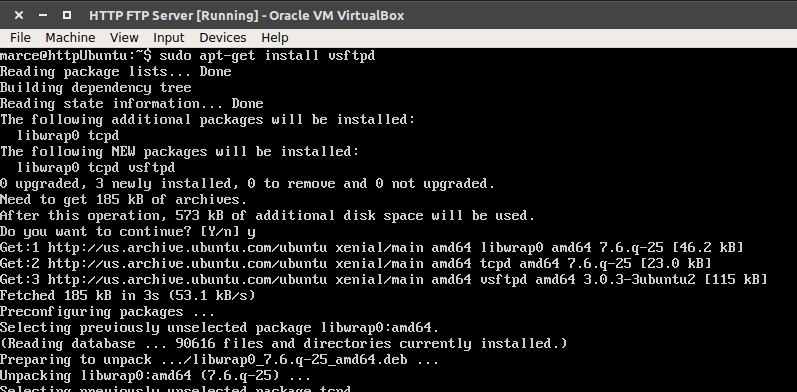
\includegraphics[width=.9 \textwidth]{images/ftp1}
		\caption{Comando de instalación FTP.}
		\label{image:ftp1}
\end{figure}
\FloatBarrier

Posteriormente, ya que se había realizado toda la descarga de paquetes, se ingreso mediante el comando \textbf{sudo nano /etc/vsftpd.conf}, como lo muestra la figura \ref{image:ftp2} con el fin de eliminar el comentario de la línea \textbf{write\_enable = YES} y de esta manera permitir la escritura de archivos dentro del servidor.

\FloatBarrier
\begin{figure}[htbp!]
		\centering
			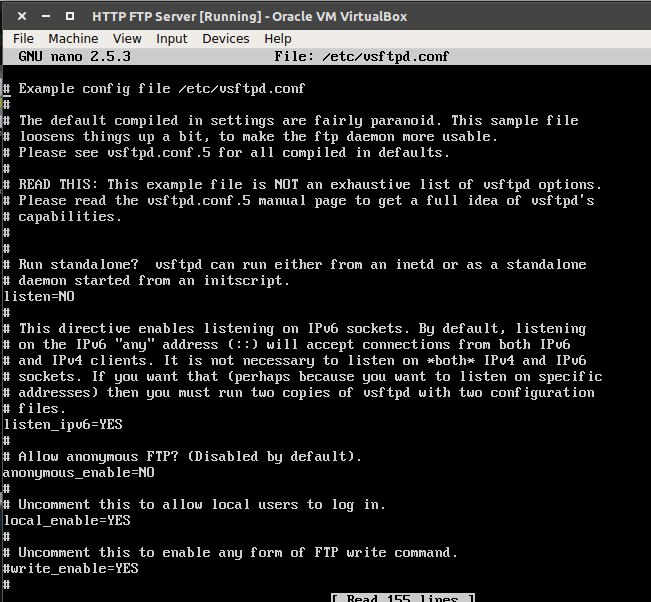
\includegraphics[width=.75 \textwidth]{images/ftp2}
		\caption{Archivo de configuración FTP.}
		\label{image:ftp2}
\end{figure}
\FloatBarrier

Por último, se ejecutó el comando \textbf{sudo service vsftp restart} con el cual se reinicia el servicio FTP y posteriormente el comando \textbf{sudo service vsftp status} para asegurarnos de que el estado del servicio sea activo. Por último únicamente se obtuvo la ip de la máquina virtual para saber el host al cual se enviarían y se recibirían los datos almacenados en dicho servidor (figura \ref{image:ftp3}).

\FloatBarrier
\begin{figure}[htbp!]
		\centering
			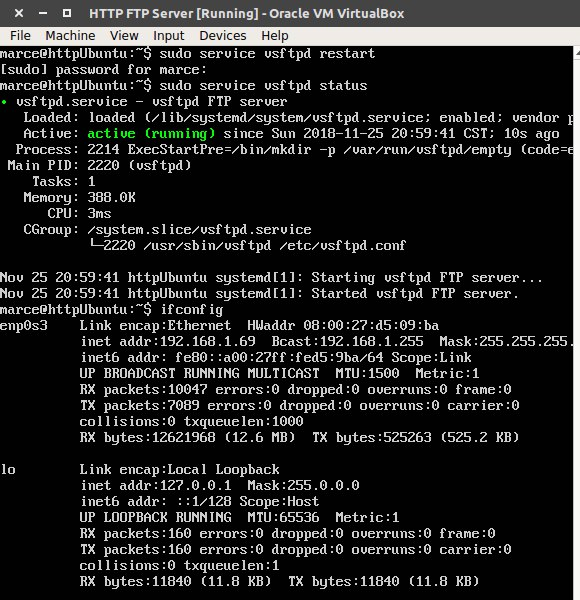
\includegraphics[width=.75 \textwidth]{images/ftp3}
		\caption{Reinicio de servicio y status FTP.}
		\label{image:ftp3}
\end{figure}
\FloatBarrier
\subsection{Sensor FTP Server File Count}

Para la implementación del contador de archivos que almacena el servidor FTP se realiza una conexión SSH y se enlistan y se cuentan los archivos en el directorio de almacenamiento del servidor. Para ello se utiliza el siguiente comando:\\
\texttt{ls -1 /home/ftp/ | wc -l}\\

El código se puede observar en la figura \ref{image:ftpcounter}.

\FloatBarrier
\begin{figure}[htbp!]
		\centering
			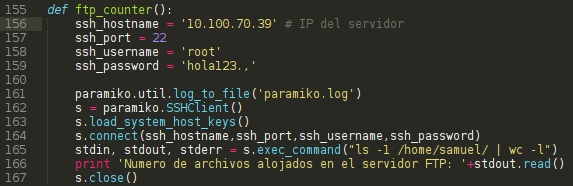
\includegraphics[width=.75 \textwidth]{images/ftpcounter}
		\caption{Código del contador de archivos en el servidor FTP.}
		\label{image:ftpcounter}
\end{figure}
\FloatBarrier

El funcionamiento se puede ver en la figura \ref{image:ftpcounterfunc}.

\FloatBarrier
\begin{figure}[htbp!]
		\centering
			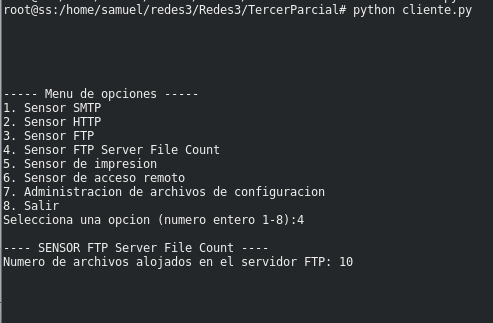
\includegraphics[width=.75 \textwidth]{images/ftpcounterfunc}
		\caption{Contador de archivos en el servidor FTP.}
		\label{image:ftpcounterfunc}
\end{figure}
\FloatBarrier